\chapter{长短时记忆网络}\label{chap:Lstm}

\begin{introduction}
	\item 长短时记忆网络是啥~\ref{Lstm:1}
	\item 长短时记忆网络的前向计算~\ref{Lstm:2}
	\item 长短时记忆网络的训练~\ref{Lstm:3}
	\item LSTM训练算法框架~\ref{Lstm:4}
	\item 关于公式和符号的说明~\ref{Lstm:5}
	\item 误差项沿时间的反向传递~\ref{Lstm:6}
	\item 将误差项传递到上一层~\ref{Lstm:7}
	\item 权重梯度的计算~\ref{Lstm:8}
	\item 编程实战:长短时记忆网络的实现~\ref{Lstm:9}
	\item 激活函数的实现~\ref{Lstm:10}
	\item LSTM初始化~\ref{Lstm:11}
	\item 前向计算的实现~\ref{Lstm:12}
	\item 反向传播算法的实现~\ref{Lstm:13}
	\item 梯度下降算法的实现~\ref{Lstm:14}
	\item 梯度检查的实现~\ref{Lstm:15}
	\item GRU~\ref{Lstm:16}
\end{introduction}

在上一篇文章中,我们介绍了\textbf{循环神经网络}以及它的训练算法。我们也介绍了\textbf{循环神经网络}很难训练的原因,这导致了它在实际应用中,很难处理长距离的依赖。在本文中,我们将介绍一种改进之后的循环神经网络:\textbf{长短时记忆网络(Long Short Term Memory Network, LSTM)},它成功的解决了原始循环神经网络的缺陷,成为当前最流行的RNN,在语音识别、图片描述、自然语言处理等许多领域中成功应用。但不幸的一面是,\textbf{LSTM}的结构很复杂,因此,我们需要花上一些力气,才能把LSTM以及它的训练算法弄明白。在搞清楚\textbf{LSTM}之后,我们再介绍一种\textbf{LSTM}的变体:\textbf{GRU (Gated Recurrent Unit)}。它的结构比\textbf{LSTM}简单,而效果却和\textbf{LSTM}一样好,因此,它正在逐渐流行起来。最后,我们仍然会动手实现一个\textbf{LSTM}。

\section{长短时记忆网络是啥}\label{Lstm:1}

我们首先了解一下长短时记忆网络产生的背景。回顾一下第\ref{chap:Cnn}章循环神经网络中推导的,误差项沿时间反向传播的公式:
\[
	\delta_k^T=\delta_t^T\prod_{i=k}^{t-1}diag[f'({net}_{i})]W
\]

我们可以根据下面的不等式,来获取\(\delta_k^T\)的模的上界(模可以看做对\(\delta_k^T\)中每一项值的大小的度量):
\begin{align*}
	\|\delta_k^T\|\leqslant & \|\delta_t^T\|\prod_{i=k}^{t-1}\|diag[f'({net}_{i})]\|\|W\| \\
	\leqslant               & \|\delta_t^T\|(\beta_f\beta_W)^{t-k}
\end{align*}

我们可以看到,误差项\(\delta\)从t时刻传递到k时刻,其值的上界是\(\beta_f\beta_w\)的指数函数。\(\beta_f\beta_w\)分别是对角矩阵\(diag[f'({net}_{i})]\)和矩阵W模的上界。显然,除非\(\beta_f\beta_w\)乘积的值位于1附近,否则,当t-k很大时(也就是误差传递很多个时刻时),整个式子的值就会变得极小(当\(\beta_f\beta_w\)乘积小于1)或者极大(当\(\beta_f\beta_w\)乘积大于1),前者就是\textbf{梯度消失},后者就是\textbf{梯度爆炸}。虽然科学家们搞出了很多技巧(比如怎样初始化权重),让\(\beta_f\beta_w\)的值尽可能贴近于1,终究还是难以抵挡指数函数的威力。

\textbf{梯度消失}到底意味着什么?在第\ref{chap:Cnn}章循环神经网络中我们已证明,权重数组W最终的梯度是各个时刻的梯度之和,即:
\begin{align*}
	\nabla_WE & =\sum_{k=1}^t\nabla_{Wk}E=\nabla_{Wt}E+\nabla_{Wt-1}E+\nabla_{Wt-2}E+...+\nabla_{W1}E
\end{align*}

假设某轮训练中,各时刻的梯度以及最终的梯度之和如图\ref{fig:Lstm1}:
\begin{figure}[!h]
	\centering
	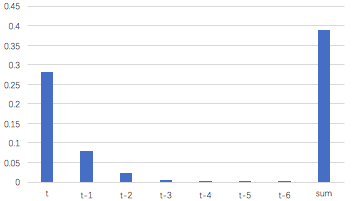
\includegraphics[width=0.7\textwidth]{Lstm1.png}
	\caption{梯度}
	\label{fig:Lstm1}
\end{figure}
我们就可以看到,从上图的t-3时刻开始,梯度已经几乎减少到0了。那么,从这个时刻开始再往之前走,得到的梯度(几乎为零)就不会对最终的梯度值有任何贡献,这就相当于无论t-3时刻之前的网络状态h是什么,在训练中都不会对权重数组W的更新产生影响,也就是网络事实上已经忽略了t-3时刻之前的状态。这就是原始RNN无法处理长距离依赖的原因。

既然找到了问题的原因,那么我们就能解决它。从问题的定位到解决,科学家们大概花了7、8年时间。终于有一天,Hochreiter和Schmidhuber两位科学家发明出\textbf{长短时记忆网络},一举解决这个问题。

其实,\textbf{长短时记忆网络}的思路比较简单。原始RNN的隐藏层只有一个状态,即h,它对于短期的输入非常敏感。那么,假如我们再增加一个状态,即c,让它来保存长期的状态,那么问题不就解决了么?如图\ref{fig:Lstm2}所示:
\begin{figure}[!h]
	\centering
	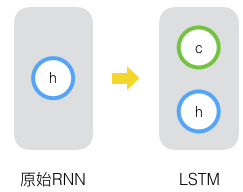
\includegraphics[width=0.35\textwidth]{Lstm2.png}
	\caption{RNN to LSTM}
	\label{fig:Lstm2}
\end{figure}

新增加的状态c,称为\textbf{单元状态(cell state)}。我们把上图按照时间维度展开:
\begin{figure}[!h]
	\centering
	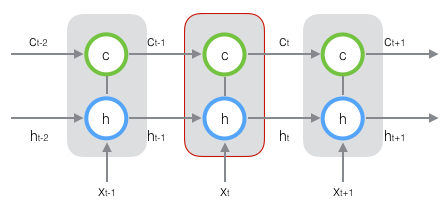
\includegraphics[width=0.7\textwidth]{Lstm3.png}
	\caption{梯度}
	\label{fig:Lstm3}
\end{figure}

图\ref{fig:Lstm3}仅仅是一个示意图,我们可以看出,在t时刻,LSTM的输入有三个:当前时刻网络的输入值\({x}_t\)、上一时刻LSTM的输出值\({h}_{t-1}\)、以及上一时刻的单元状态\({c}_{t-1}\);LSTM的输出有两个:当前时刻LSTM输出值\({h}_t\)、和当前时刻的单元状态\({c}_t\)。注意\({x}\)、\({h}\)、\({c}\)都是\textbf{向量}。

LSTM的关键,就是怎样控制长期状态c。在这里,LSTM的思路是使用三个控制开关。第一个开关,负责控制继续保存长期状态c;第二个开关,负责控制把即时状态输入到长期状态c;第三个开关,负责控制是否把长期状态c作为当前的LSTM的输出。三个开关的作用如图\ref{fig:Lstm4}所示:

\begin{figure}[!h]
	\centering
	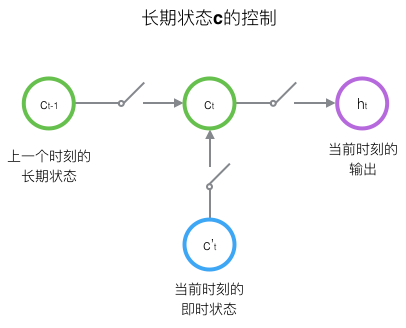
\includegraphics[width=0.6\textwidth]{Lstm4.png}
	\caption{梯度}
	\label{fig:Lstm4}
\end{figure}


接下来,我们要描述一下,输出h和单元状态c的具体计算方法。

\section{长短时记忆网络的前向计算}\label{Lstm:2}

前面描述的开关是怎样在算法中实现的呢?这就用到了\textbf{门(gate)}的概念。门实际上就是一层\textbf{全连接层},它的输入是一个向量,输出是一个0到1之间的实数向量。假设W是门的权重向量,\({b}\)是偏置项,那么门可以表示为:
\[
	g({x})=\sigma(W{x}+{b})
\]

门的使用,就是用门的输出向量按元素乘以我们需要控制的那个向量。因为门的输出是0到1之间的实数向量,那么,当门输出为0时,任何向量与之相乘都会得到0向量,这就相当于啥都不能通过;输出为1时,任何向量与之相乘都不会有任何改变,这就相当于啥都可以通过。因为\(\sigma\)(也就是sigmoid函数)的值域是(0,1),所以门的状态都是半开半闭的。

LSTM用两个门来控制单元状态c的内容,一个是\textbf{遗忘门(forget gate)},它决定了上一时刻的单元状态\({c}_{t-1}\)有多少保留到当前时刻\({c}_t\);另一个是\textbf{输入门(input gate)},它决定了当前时刻网络的输入\({x}_t\)有多少保存到单元状态\({c}_t\)。LSTM用\textbf{输出门(output gate)}来控制单元状态\({c}_t\)有多少输出到LSTM的当前输出值\({h}_t\)。

我们先来看一下遗忘门:
\begin{equation}
	\label{eq:Lstm1}
	{f}_t=\sigma(W_f\cdot[{h}_{t-1},{x}_t]+{b}_f)
\end{equation}
上式中,\(W_f\)是遗忘门的权重矩阵,\([{h}_{t-1},{x}_t]\)表示把两个向量连接成一个更长的向量,\({b}_f\)是遗忘门的偏置项,\(\sigma\)是sigmoid函数。如果输入的维度是\(d_x\),隐藏层的维度是\(d_h\),单元状态的维度是\(d_c\)(通常\(d_c=d_h\)),则遗忘门的权重矩阵\(W_f\)维度是\( d_c\times (d_h+d_x)\)。事实上,权重矩阵\(W_f\)都是两个矩阵拼接而成的:一个是\(W_{fh}\),它对应着输入项\({h}_{t-1}\),其维度为\(d_c\times d_h\);一个是\(W_{fx}\),它对应着输入项\({x}_t\),其维度为\(d_c\times d_x\)。\(W_f\)可以写为:
\begin{align*}
	\begin{bmatrix}W_f\end{bmatrix}\begin{bmatrix}{h}_{t-1} \\
		{x}_t\end{bmatrix} & =\begin{bmatrix}W_{fh}&W_{fx}\end{bmatrix}\begin{bmatrix}{h}_{t-1} \\
		{x}_t\end{bmatrix} \\
	                                                    & =W_{fh}{h}_{t-1}+W_{fx}{x}_t
\end{align*}

图\ref{fig:Lstm5}显示了遗忘门的计算:
\begin{figure}[!h]
	\centering
	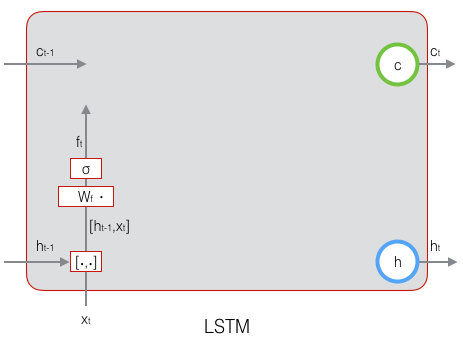
\includegraphics[width=0.6\textwidth]{Lstm5.png}
	\caption{遗忘门}
	\label{fig:Lstm5}
\end{figure}

接下来看看输入门:
\begin{equation}
	\label{eq:Lstm2}
	{i}_t=\sigma(W_i\cdot[{h}_{t-1},{x}_t]+{b}_i)
\end{equation}
上式中,\(W_i\)是输入门的权重矩阵,\({b}_i\)是输入门的偏置项。图\ref{fig:Lstm6}表示了输入门的计算:
\begin{figure}[!h]
	\centering
	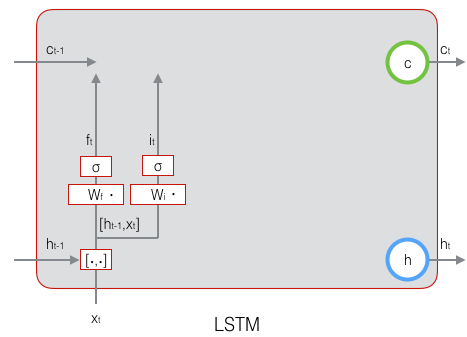
\includegraphics[width=0.6\textwidth]{Lstm6.png}
	\caption{输入门}
	\label{fig:Lstm6}
\end{figure}

接下来,我们计算用于描述当前输入的单元状态\({\tilde{c}}_t\),它是根据上一次的输出和本次输入来计算的:
\begin{equation}
	\label{eq:Lstm3}
	{\tilde{c}}_t=\tanh(W_c\cdot[{h}_{t-1},{x}_t]+{b}_c)
\end{equation}

图\ref{fig:Lstm7}是\({\tilde{c}}_t\)的计算:
\begin{figure}[!h]
	\centering
	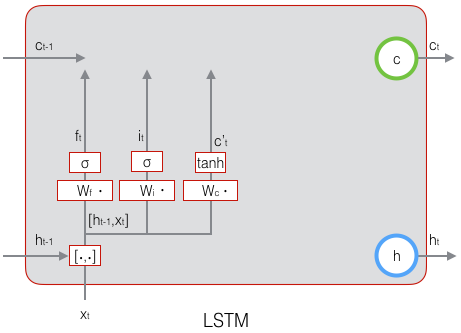
\includegraphics[width=0.6\textwidth]{Lstm7.png}
	\caption{\({\tilde{c}}_t\)的计算}
	\label{fig:Lstm7}
\end{figure}
现在,我们计算当前时刻的单元状态\({c}_t\)。它是由上一次的单元状态\({c}_{t-1}\)按元素乘以遗忘门\(f_t\),再用当前输入的单元状态\({\tilde{c}}_t\)按元素乘以输入门\(i_t\),再将两个积加和产生的:
\begin{equation}
	\label{eq:Lstm4}
	{c}_t=f_t\circ{{c}_{t-1}}+i_t\circ{{\tilde{c}}_t}
\end{equation}
符号\(\circ\)表示\textbf{按元素乘}。图\ref{fig:Lstm8}是\({c}_t\)的计算:

\begin{figure}[!h]
	\centering
	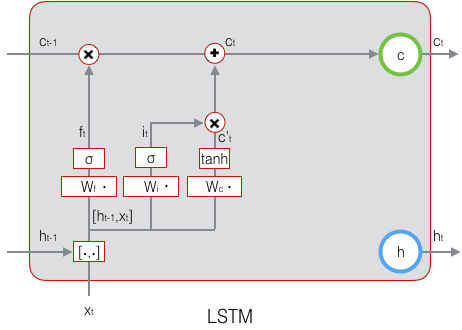
\includegraphics[width=0.6\textwidth]{Lstm8.png}
	\caption{\({c}_t\)的计算}
	\label{fig:Lstm8}
\end{figure}

这样,我们就把LSTM关于当前的记忆\({\tilde{c}}_t\)和长期的记忆\({c}_{t-1}\)组合在一起,形成了新的单元状态\({c}_t\)。由于遗忘门的控制,它可以保存很久很久之前的信息,由于输入门的控制,它又可以避免当前无关紧要的内容进入记忆。下面,我们要看看输出门,它控制了长期记忆对当前输出的影响:
\begin{equation}
	\label{eq:Lstm5}
	{o}_t=\sigma(W_o\cdot[{h}_{t-1},{x}_t]+{b}_o)
\end{equation}

图\ref{fig:Lstm9}表示输出门的计算:

\begin{figure}[!h]
	\centering
	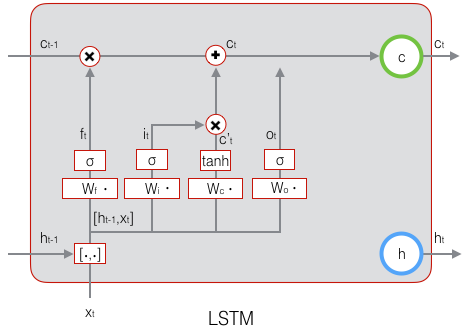
\includegraphics[width=0.6\textwidth]{Lstm9.png}
	\caption{输出门}
	\label{fig:Lstm9}
\end{figure}

LSTM最终的输出,是由输出门和单元状态共同确定的:
\begin{equation}
	\label{eq:Lstm6}
	{h}_t={o}_t\circ \tanh({c}_t)
\end{equation}

图\ref{fig:Lstm10}表示LSTM最终输出的计算。

\begin{figure}[!h]
	\centering
	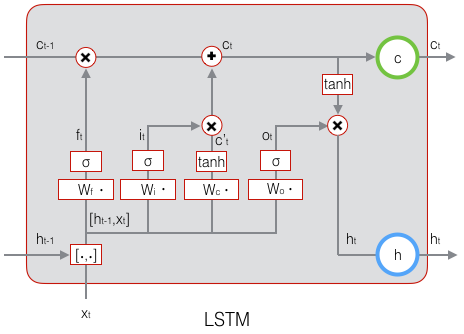
\includegraphics[width=0.6\textwidth]{Lstm10.png}
	\caption{LSTM最终输出}
	\label{fig:Lstm10}
\end{figure}

公式\ref{eq:Lstm1}到公式\ref{eq:Lstm6}就是LSTM前向计算的全部公式。至此,我们就把LSTM前向计算讲完了。

\section{长短时记忆网络的训练}\label{Lstm:3}

熟悉我们这个系列文章的同学都清楚,训练部分往往比前向计算部分复杂多了。
{LSTM} 的前向计算都这么复杂,那么,可想而知,它的训练算法一定是非常非常复杂的。
现在只有做几次深呼吸,再一头扎进公式海洋吧。

\subsection{LSTM训练算法框架}\label{Lstm:4}

LSTM的训练算法仍然是反向传播算法,对于这个算法,我们已经非常熟悉了。主要有下面三个步骤:

\begin{enumerate}
	\item
	      前向计算每个神经元的输出值,对于LSTM来说,即\({f}_t\)、\({i}_t\)、\({c}_t\)、\({o}_t\)、\({h}_t\)五个向量的值。计算方法已经在上一节中描述过了。
	\item
	      反向计算每个神经元的\textbf{误差项}\(\delta\)值。与\textbf{循环神经网络}一样,LSTM误差项的反向传播也是包括两个方向:一个是沿时间的反向传播,即从当前t时刻开始,计算每个时刻的误差项;一个是将误差项向上一层传播。
	\item
	      根据相应的误差项,计算每个权重的梯度。
\end{enumerate}


\subsection{关于公式和符号的说明}\label{Lstm:5}

首先,我们对推导中用到的一些公式、符号做一下必要的说明。

接下来的推导中,我们设定gate的激活函数为sigmoid函数,输出的激活函数为tanh函数。他们的导数分别为:
\begin{align*}
	\sigma(z)  & =y=\frac{1}{1+e^{-z}}            \\
	\sigma'(z) & =y(1-y)                          \\
	\tanh(z)   & =y=\frac{e^z-e^{-z}}{e^z+e^{-z}} \\
	\tanh'(z)  & =1-y^2
\end{align*}

从上面可以看出,sigmoid和tanh函数的导数都是原函数的函数。这样,我们一旦计算原函数的值,就可以用它来计算出导数的值。

LSTM需要学习的参数共有8组,分别是:遗忘门的权重矩阵\(W_f\)和偏置项\({b}_f\)、输入门的权重矩阵\(W_i\)和偏置项\({b}_i\)、输出门的权重矩阵\(W_o\)和偏置项\({b}_o\),以及计算单元状态的权重矩阵\(W_c\)和偏置项\({b}_c\)。因为权重矩阵的两部分在反向传播中使用不同的公式,因此在后续的推导中,权重矩阵\(W_f\)、\(W_i\)、\(W_c\)、\(W_o\)都将被写为分开的两个矩阵:\(W_{fh}\)、\(W_{fx}\)、\(W_{ih}\)、\(W_{ix}\)、\(W_{oh}\)、\(W_{ox}\)、\(W_{ch}\)、\(W_{cx}\)。

我们解释一下按元素乘\(\circ\)符号。当\(\circ\)作用于两个\textbf{向量}时,运算如下:
\[
	{a}\circ{b}=\begin{bmatrix}
		a_1 \\a_2\\a_3\\...\\a_n
	\end{bmatrix}\circ\begin{bmatrix}
		b_1 \\b_2\\b_3\\...\\b_n
	\end{bmatrix}=\begin{bmatrix}
		a_1b_1 \\a_2b_2\\a_3b_3\\...\\a_nb_n
	\end{bmatrix}
\]

当\(\circ\)作用于一个\textbf{向量}和一个\textbf{矩阵}时,运算如下:
\begin{align*}
	{a}\circ X & =\begin{bmatrix}
		a_1 \\a_2\\a_3\\...\\a_n
	\end{bmatrix}\circ\begin{bmatrix}
		x_{11} & x_{12} & x_{13} & ... & x_{1n} \\
		x_{21} & x_{22} & x_{23} & ... & x_{2n} \\
		x_{31} & x_{32} & x_{33} & ... & x_{3n} \\
		       &        & ...                   \\
		x_{n1} & x_{n2} & x_{n3} & ... & x_{nn} \\
	\end{bmatrix} \\
	           & =\begin{bmatrix}
		a_1x_{11} & a_1x_{12} & a_1x_{13} & ... & a_1x_{1n} \\
		a_2x_{21} & a_2x_{22} & a_2x_{23} & ... & a_2x_{2n} \\
		a_3x_{31} & a_3x_{32} & a_3x_{33} & ... & a_3x_{3n} \\
		          &           & ...                         \\
		a_nx_{n1} & a_nx_{n2} & a_nx_{n3} & ... & a_nx_{nn} \\
	\end{bmatrix}
\end{align*}

当\(\circ\)作用于两个\textbf{矩阵}时,两个矩阵对应位置的元素相乘。按元素乘可以在某些情况下简化矩阵和向量运算。例如,当一个对角矩阵右乘一个矩阵时,相当于用对角矩阵的对角线组成的向量按元素乘那个矩阵:
\[
	diag[{a}]X={a}\circ X
\]

当一个行向量右乘一个对角矩阵时,相当于这个行向量按元素乘那个矩阵对角线组成的向量:
\[
	{a}^Tdiag[{b}]={a}\circ{b}
\]

上面这两点,在我们后续推导中会多次用到。

在t时刻,LSTM的输出值为\({h}_t\)。我们定义t时刻的误差项\(\delta_t\)为:
\[
	\delta_t\overset{def}{=}\frac{\partial{E}}{\partial{{h}_t}}
\]

注意,和前面几篇文章不同,我们这里假设误差项是损失函数对输出值的导数,而不是对加权输入\(net_t^l\)的导数。因为LSTM有四个加权输入,分别对应\({f}_t\)、\({i}_t\)、\({c}_t\)、\({o}_t\),我们希望往上一层传递一个误差项而不是四个。但我们仍然需要定义出这四个加权输入,以及他们对应的误差项。

\begin{align*}
	{net}_{f,t}         & =W_f[{h}_{t-1},{x}_t]+{b}_f=W_{fh}{h}_{t-1}+W_{fx}{x}_t+{b}_f                                                                                                                                                                                                                                  \\
	{net}_{i,t}         & =W_i[{h}_{t-1},{x}_t]+{b}_i=W_{ih}{h}_{t-1}+W_{ix}{x}_t+{b}_i                                                                                                                                                                                                                                  \\
	{net}_{\tilde{c},t} & =W_c[{h}_{t-1},{x}_t]+{b}_c=W_{ch}{h}_{t-1}+W_{cx}{x}_t+{b}_c                                                                                                                                                                                                                                  \\
	{net}_{o,t}         & =W_o[{h}_{t-1},{x}_t]+{b}_o=W_{oh}{h}_{t-1}+W_{ox}{x}_t+{b}_o                                                                                                                                                                                                                                  \\
	\delta_{f,t}        & \overset{def}{=}\frac{\partial{E}}{\partial{{net}_{f,t}}}, \delta_{i,t}\overset{def}{=}\frac{\partial{E}}{\partial{{net}_{i,t}}}, \delta_{\tilde{c},t}\overset{def}{=}\frac{\partial{E}}{\partial{{net}_{\tilde{c},t}}}, \delta_{o,t}\overset{def}{=}\frac{\partial{E}}{\partial{{net}_{o,t}}}
\end{align*}

\subsection{误差项沿时间的反向传递}\label{Lstm:6}

沿时间反向传递误差项,就是要计算出t-1时刻的误差项\(\delta_{t-1}\)。
\begin{align*}
	\delta_{t-1}^T=\frac{\partial{E}}{\partial{{h_{t-1}}}}=\frac{\partial{E}}{\partial{{h_t}}}\frac{\partial{{h_t}}}{\partial{{h_{t-1}}}}=\delta_{t}^T\frac{\partial{{h_t}}}{\partial{{h_{t-1}}}}
\end{align*}

我们知道,\(\frac{\partial{{h_t}}}{\partial{{h_{t-1}}}}\)是一个Jacobian矩阵。如果隐藏层h的维度是N的话,那么它就是一个\(N\times N\)矩阵。为了求出它,我们列出\({h}_t\)的计算公式,即前面的公式\ref{eq:Lstm4}和公式\ref{eq:Lstm6}:
\begin{align*}
	{h}_t & ={o}_t\circ \tanh({c}_t)                     \\
	{c}_t & ={f}_t\circ{c}_{t-1}+{i}_t\circ{\tilde{c}}_t
\end{align*}

显然,\({o}_t\)、\({f}_t\)、\({i}_t\)、\({\tilde{c}}_t\)都是\({h}_{t-1}\)的函数,那么,利用全导数公式可得:
\begin{align}
	\delta_t^T\frac{\partial{{h_t}}}{\partial{{h_{t-1}}}} & =\delta_t^T\frac{\partial{{h_t}}}{\partial{{o}_t}}\frac{\partial{{o}_t}}{\partial{{net}_{o,t}}}\frac{\partial{{net}_{o,t}}}{\partial{{h_{t-1}}}}
	+\delta_t^T\frac{\partial{{h_t}}}{\partial{{c}_t}}\frac{\partial{{c}_t}}{\partial{{f_{t}}}}\frac{\partial{{f}_t}}{\partial{{net}_{f,t}}}\frac{\partial{{net}_{f,t}}}{\partial{{h_{t-1}}}}\notag                                                   \\
	                                                      & +\delta_t^T\frac{\partial{{h_t}}}{\partial{{c}_t}}\frac{\partial{{c}_t}}{\partial{{i_{t}}}}\frac{\partial{{i}_t}}{\partial{{net}_{i,t}}}\frac{\partial{{net}_{i,t}}}{\partial{{h_{t-1}}}}
	+\delta_t^T\frac{\partial{{h_t}}}{\partial{{c}_t}}\frac{\partial{{c}_t}}{\partial{{\tilde{c}}_{t}}}\frac{\partial{{\tilde{c}}_t}}{\partial{{net}_{\tilde{c},t}}}\frac{\partial{{net}_{\tilde{c},t}}}{\partial{{h_{t-1}}}}\notag                   \\
	                                                      & =\delta_{o,t}^T\frac{\partial{{net}_{o,t}}}{\partial{{h_{t-1}}}}
	+\delta_{f,t}^T\frac{\partial{{net}_{f,t}}}{\partial{{h_{t-1}}}}
	+\delta_{i,t}^T\frac{\partial{{net}_{i,t}}}{\partial{{h_{t-1}}}}
	+\delta_{\tilde{c},t}^T\frac{\partial{{net}_{\tilde{c},t}}}{\partial{{h_{t-1}}}}\label{eq:Lstm7}
\end{align}


下面,我们要把公式\ref{eq:Lstm7}中的每个偏导数都求出来。根据公式\ref{eq:Lstm6},我们可以求出:
\begin{align*}
	\frac{\partial{{h_t}}}{\partial{{o}_t}} & =diag[\tanh({c}_t)]                 \\
	\frac{\partial{{h_t}}}{\partial{{c}_t}} & =diag[{o}_t\circ(1-\tanh({c}_t)^2)]
\end{align*}

根据公式\ref{eq:Lstm4},我们可以求出:
\begin{align*}
	\frac{\partial{{c}_t}}{\partial{{f_{t}}}}=diag[{c}_{t-1}],\quad
	\frac{\partial{{c}_t}}{\partial{{i_{t}}}}=diag[{\tilde{c}}_t],\quad
	\frac{\partial{{c}_t}}{\partial{{\tilde{c}_{t}}}}=diag[{i}_t]
\end{align*}

因为:
\begin{align*}
	{o}_t         & =\sigma({net}_{o,t}),\quad {net}_{o,t}=W_{oh}{h}_{t-1}+W_{ox}{x}_t+{b}_o                \\
	{f}_t         & =\sigma({net}_{f,t}),\quad {net}_{f,t}=W_{fh}{h}_{t-1}+W_{fx}{x}_t+{b}_f                \\
	{i}_t         & =\sigma({net}_{i,t}),\quad {net}_{i,t}=W_{ih}{h}_{t-1}+W_{ix}{x}_t+{b}_i                \\
	{\tilde{c}}_t & =\tanh({net}_{\tilde{c},t}),\quad {net}_{\tilde{c},t}=W_{ch}{h}_{t-1}+W_{cx}{x}_t+{b}_c
\end{align*}

我们很容易得出:
\begin{align*}
	\frac{\partial{{o}_t}}{\partial{{net}_{o,t}}}                 & =diag[{o}_t\circ(1-{o}_t)],\quad \frac{\partial{{net}_{o,t}}}{\partial{{h_{t-1}}}}=W_{oh}       \\
	\frac{\partial{{f}_t}}{\partial{{net}_{f,t}}}                 & =diag[{f}_t\circ(1-{f}_t)],\quad \frac{\partial{{net}_{f,t}}}{\partial{{h}_{t-1}}}=W_{fh}       \\
	\frac{\partial{{i}_t}}{\partial{{net}_{i,t}}}                 & =diag[{i}_t\circ(1-{i}_t)],\quad \frac{\partial{{net}_{i,t}}}{\partial{{h}_{t-1}}}=W_{ih}       \\
	\frac{\partial{{\tilde{c}}_t}}{\partial{{net}_{\tilde{c},t}}} & =diag[1-{\tilde{c}}_t^2],\quad \frac{\partial{{net}_{\tilde{c},t}}}{\partial{{h}_{t-1}}}=W_{ch}
\end{align*}

将上述偏导数带入到公式\ref{eq:Lstm7},我们得到:
\begin{align}
	\delta_{t-1} & =\delta_{o,t}^T\frac{\partial{{net}_{o,t}}}{\partial{{h_{t-1}}}}
	+\delta_{f,t}^T\frac{\partial{{net}_{f,t}}}{\partial{{h_{t-1}}}}
	+\delta_{i,t}^T\frac{\partial{{net}_{i,t}}}{\partial{{h_{t-1}}}}
	+\delta_{\tilde{c},t}^T\frac{\partial{{net}_{\tilde{c},t}}}{\partial{{h_{t-1}}}}\notag \\
	             & =\delta_{o,t}^T W_{oh}
	+\delta_{f,t}^TW_{fh}
	+\delta_{i,t}^TW_{ih}
	+\delta_{\tilde{c},t}^TW_{ch}\label{eq:Lstm8}
\end{align}

根据\(\delta_{o,t}\)、\(\delta_{f,t}\)、\(\delta_{i,t}\)、\(\delta_{\tilde{c},t}\)的定义,可知:
\begin{align}
	\delta_{o,t}^T         & =\delta_t^T\circ\tanh({c}_t)\circ{o}_t\circ(1-{o}_t)\label{eq:Lstm9}                                    \\
	\delta_{f,t}^T         & =\delta_t^T\circ{o}_t\circ(1-\tanh({c}_t)^2)\circ{c}_{t-1}\circ{f}_t\circ(1-{f}_t)\label{eq:Lstm10}     \\
	\delta_{i,t}^T         & =\delta_t^T\circ{o}_t\circ(1-\tanh({c}_t)^2)\circ{\tilde{c}}_t\circ{i}_t\circ(1-{i}_t)\label{eq:Lstm11} \\
	\delta_{\tilde{c},t}^T & =\delta_t^T\circ{o}_t\circ(1-\tanh({c}_t)^2)\circ{i}_t\circ(1-{\tilde{c}}^2)\label{eq:Lstm12}
\end{align}

公式\ref{eq:Lstm8}到公式\ref{eq:Lstm12}就是将误差沿时间反向传播一个时刻的公式。有了它,我们可以写出将误差项向前传递到任意k时刻的公式:
\begin{equation}
	\label{eq:Lstm13}
	\delta_k^T=\prod_{j=k}^{t-1}\delta_{o,j}^TW_{oh}
	+\delta_{f,j}^TW_{fh}
	+\delta_{i,j}^TW_{ih}
	+\delta_{\tilde{c},j}^TW_{ch}
\end{equation}

\subsection{将误差项传递到上一层}\label{Lstm:7}

我们假设当前为第l层,定义l-1层的误差项是误差函数对l-1层\textbf{加权输入}的导数,即:
\[
	\delta_t^{l-1}\overset{def}{=}\frac{\partial{E}}{{net}_t^{l-1}}
\]

本次LSTM的输入\(x_t\)由下面的公式计算:
\[
	{x}_t^l=f^{l-1}({net}_t^{l-1})
\]
上式中,\(f^{l-1}\)表示第l-1层的\textbf{激活函数}。

因为\({net}_{f,t}^l\)、\({net}_{i,t}^l\)、\({net}_{\tilde{c},t}^l\)、\({net}_{o,t}^l\)都是\({x}_t\)的函数,\({x}_t\)又是\({net}_t^{l-1}\)的函数,因此,要求出E对\({net}_t^{l-1}\)的导数,就需要使用全导数公式:

\begin{align}
	\frac{\partial{E}}{\partial{{net}_t^{l-1}}} & =\frac{\partial{E}}{\partial{{{net}_{f,t}^l}}}\frac{\partial{{{net}_{f,t}^l}}}{\partial{{x}_t^l}}\frac{\partial{{x}_t^l}}{\partial{{{net}_t^{l-1}}}}
	+\frac{\partial{E}}{\partial{{{net}_{i,t}^l}}}\frac{\partial{{{net}_{i,t}^l}}}{\partial{{x}_t^l}}\frac{\partial{{x}_t^l}}{\partial{{{net}_t^{l-1}}}}
	\notag                                                                                                                                                                                                                                       \\&+\frac{\partial{E}}{\partial{{{net}_{\tilde{c},t}^l}}}\frac{\partial{{{net}_{\tilde{c},t}^l}}}{\partial{{x}_t^l}}\frac{\partial{{x}_t^l}}{\partial{{{net}_t^{l-1}}}}
	+\frac{\partial{E}}{\partial{{{net}_{o,t}^l}}}\frac{\partial{{{net}_{o,t}^l}}}{\partial{{x}_t^l}}\frac{\partial{{x}_t^l}}{\partial{{{net}_t^{l-1}}}}\notag                                                                                   \\
	                                            & =\delta_{f,t}^TW_{fx}\circ f'({net}_t^{l-1})+\delta_{i,t}^TW_{ix}\circ f'({net}_t^{l-1})+\delta_{\tilde{c},t}^TW_{cx}\circ f'({net}_t^{l-1})+\delta_{o,t}^TW_{ox}\circ f'({net}_t^{l-1})\notag \\
	                                            & =(\delta_{f,t}^TW_{fx}+\delta_{i,t}^TW_{ix}+\delta_{\tilde{c},t}^TW_{cx}+\delta_{o,t}^TW_{ox})\circ f'({net}_t^{l-1})\label{eq:Lstm14}
\end{align}

公式\ref{eq:Lstm14}就是将误差传递到上一层的公式。



\subsection{权重梯度的计算}\label{Lstm:8}

对于\(W_{fh}\)、\(W_{ih}\)、\(W_{ch}\)、\(W_{oh}\)的权重梯度,我们知道它的梯度是各个时刻梯度之和(证明过程请参考第\ref{chap:Rnn}循环神经网络),我们首先求出它们在t时刻的梯度,然后再求出他们最终的梯度。

我们已经求得了误差项\(\delta_{o,t}\)、\(\delta_{f,t}\)、\(\delta_{i,t}\)、\(\delta_{\tilde{c},t}\),很容易求出t时刻的\(W_{oh}\)、的\(W_{ih}\)、的\(W_{fh}\)、的\(W_{ch}\):
\begin{align*}
	\frac{\partial{E}}{\partial{W_{oh,t}}} & =\frac{\partial{E}}{\partial{{net}_{o,t}}}\frac{\partial{{net}_{o,t}}}{\partial{W_{oh,t}}}=\delta_{o,t}{h}_{t-1}^T                         \\
	\frac{\partial{E}}{\partial{W_{fh,t}}} & =\frac{\partial{E}}{\partial{{net}_{f,t}}}\frac{\partial{{net}_{f,t}}}{\partial{W_{fh,t}}}=\delta_{f,t}{h}_{t-1}^T                         \\
	\frac{\partial{E}}{\partial{W_{ih,t}}} & =\frac{\partial{E}}{\partial{{net}_{i,t}}}\frac{\partial{{net}_{i,t}}}{\partial{W_{ih,t}}}=\delta_{i,t}{h}_{t-1}^T                         \\
	\frac{\partial{E}}{\partial{W_{ch,t}}} & =\frac{\partial{E}}{\partial{{net}_{\tilde{c},t}}}\frac{\partial{{net}_{\tilde{c},t}}}{\partial{W_{ch,t}}}=\delta_{\tilde{c},t}{h}_{t-1}^T
\end{align*}

将各个时刻的梯度加在一起,就能得到最终的梯度:
\begin{align*}
	\frac{\partial{E}}{\partial{W_{oh}}} & =\sum_{j=1}^t\delta_{o,j}{h}_{j-1}^T         \\
	\frac{\partial{E}}{\partial{W_{fh}}} & =\sum_{j=1}^t\delta_{f,j}{h}_{j-1}^T         \\
	\frac{\partial{E}}{\partial{W_{ih}}} & =\sum_{j=1}^t\delta_{i,j}{h}_{j-1}^T         \\
	\frac{\partial{E}}{\partial{W_{ch}}} & =\sum_{j=1}^t\delta_{\tilde{c},j}{h}_{j-1}^T
\end{align*}

对于偏置项\({b}_f\)、\({b}_i\)、\({b}_c\)、\({b}_o\)的梯度,也是将各个时刻的梯度加在一起。下面是各个时刻的偏置项梯度:
\begin{align*}
	\frac{\partial{E}}{\partial{{b}_{o,t}}} & =\frac{\partial{E}}{\partial{{net}_{o,t}}}\frac{\partial{{net}_{o,t}}}{\partial{{b}_{o,t}}}=\delta_{o,t}                         \\
	\frac{\partial{E}}{\partial{{b}_{f,t}}} & =\frac{\partial{E}}{\partial{{net}_{f,t}}}\frac{\partial{{net}_{f,t}}}{\partial{{b}_{f,t}}}=\delta_{f,t}                         \\
	\frac{\partial{E}}{\partial{{b}_{i,t}}} & =\frac{\partial{E}}{\partial{{net}_{i,t}}}\frac{\partial{{net}_{i,t}}}{\partial{{b}_{i,t}}}=\delta_{i,t}                         \\
	\frac{\partial{E}}{\partial{{b}_{c,t}}} & =\frac{\partial{E}}{\partial{{net}_{\tilde{c},t}}}\frac{\partial{{net}_{\tilde{c},t}}}{\partial{{b}_{c,t}}}=\delta_{\tilde{c},t}
\end{align*}

下面是最终的偏置项梯度,即将各个时刻的偏置项梯度加在一起:
\begin{align*}
	\frac{\partial{E}}{\partial{{b}_o}}=\sum_{j=1}^t\delta_{o,j},
	\frac{\partial{E}}{\partial{{b}_i}}=\sum_{j=1}^t\delta_{i,j},
	\frac{\partial{E}}{\partial{{b}_f}}=\sum_{j=1}^t\delta_{f,j},
	\frac{\partial{E}}{\partial{{b}_c}}=\sum_{j=1}^t\delta_{\tilde{c},j}
\end{align*}

对于\(W_{fx}\)、\(W_{ix}\)、\(W_{cx}\)、\(W_{ox}\)的权重梯度,只需要根据相应的误差项直接计算即可:
\begin{align*}
	\frac{\partial{E}}{\partial{W_{ox}}} & =\frac{\partial{E}}{\partial{{net}_{o,t}}}\frac{\partial{{net}_{o,t}}}{\partial{W_{ox}}}=\delta_{o,t}{x}_{t}^T                         \\
	\frac{\partial{E}}{\partial{W_{fx}}} & =\frac{\partial{E}}{\partial{{net}_{f,t}}}\frac{\partial{{net}_{f,t}}}{\partial{W_{fx}}}=\delta_{f,t}{x}_{t}^T                         \\
	\frac{\partial{E}}{\partial{W_{ix}}} & =\frac{\partial{E}}{\partial{{net}_{i,t}}}\frac{\partial{{net}_{i,t}}}{\partial{W_{ix}}}=\delta_{i,t}{x}_{t}^T                         \\
	\frac{\partial{E}}{\partial{W_{cx}}} & =\frac{\partial{E}}{\partial{{net}_{\tilde{c},t}}}\frac{\partial{{net}_{\tilde{c},t}}}{\partial{W_{cx}}}=\delta_{\tilde{c},t}{x}_{t}^T
\end{align*}

以上就是LSTM的训练算法的全部公式。因为这里面存在很多重复的模式,仔细看看,会发觉并不是太复杂。

当然,LSTM存在着相当多的变体,读者可以在互联网上找到很多资料。因为大家已经熟悉了基本LSTM的算法,因此理解这些变体比较容易,因此本文就不再赘述了。




\section{编程实战:长短时记忆网络的实现}\label{Lstm:9}

\begin{note}
	完整代码请参考GitHub: \url{https://github.com/hanbt/learn_dl/blob/master/lstm.py}
	(python2.7)
\end{note}

在下面的实现中,LSTMLayer的参数包括输入维度、输出维度、隐藏层维度,单元状态维度等于隐藏层维度。gate的激活函数为sigmoid函数,输出的激活函数为tanh。

\subsection{激活函数的实现}\label{Lstm:10}
我们先实现两个激活函数:sigmoid和tanh。
\begin{lstlisting}
class SigmoidActivator(object):
    def forward(self, weighted_input):
        return 1.0 / (1.0 + np.exp(-weighted_input))
    def backward(self, output):
        return output * (1 - output)
class TanhActivator(object):
    def forward(self, weighted_input):
        return 2.0 / (1.0 + np.exp(-2 * weighted_input)) - 1.0
    def backward(self, output):
        return 1 - output * output
\end{lstlisting}


\subsection{LSTM初始化}\label{Lstm:11}

和前两篇文章代码架构一样,我们把LSTM的实现放在LstmLayer类中。

根据LSTM前向计算和方向传播算法,我们需要初始化一系列矩阵和向量。这些矩阵和向量有两类用途,一类是用于保存模型参数,例如\(W_f\)、\(W_i\)、\(W_o\)、\(W_c\)、\({b}_f\)、\({b}_i\)、\({b}_o\)、\({b}_c\);另一类是保存各种中间计算结果,以便于反向传播算法使用,它们包括\({h}_t\)、\({f}_t\)、\({i}_t\)、\({o}_t\)、\({c}_t\)、\({\tilde{c}}_t\)、\(\delta_t\)、\(\delta_{f,t}\)、\(\delta_{i,t}\)、\(\delta_{o,t}\)、\(\delta_{\tilde{c},t}\),以及各个权重对应的梯度。

在构造函数的初始化中,只初始化了与forward计算相关的变量,与backward相关的变量没有初始化。这是因为构造LSTM对象的时候,我们还不知道它未来是用于训练(既有forward又有backward)还是推理(只有forward)。
\begin{lstlisting}
class LstmLayer(object):
    def __init__(self, input_width, state_width, 
                 learning_rate):
        self.input_width = input_width
        self.state_width = state_width
        self.learning_rate = learning_rate
        # 门的激活函数
        self.gate_activator = SigmoidActivator()
        # 输出的激活函数
        self.output_activator = TanhActivator()
        # 当前时刻初始化为t0
        self.times = 0       
        # 各个时刻的单元状态向量c
        self.c_list = self.init_state_vec()
        # 各个时刻的输出向量h
        self.h_list = self.init_state_vec()
        # 各个时刻的遗忘门f
        self.f_list = self.init_state_vec()
        # 各个时刻的输入门i
        self.i_list = self.init_state_vec()
        # 各个时刻的输出门o
        self.o_list = self.init_state_vec()
        # 各个时刻的即时状态c~
        self.ct_list = self.init_state_vec()
        # 遗忘门权重矩阵Wfh, Wfx, 偏置项bf
        self.Wfh, self.Wfx, self.bf = (
            self.init_weight_mat())
        # 输入门权重矩阵Wfh, Wfx, 偏置项bf
        self.Wih, self.Wix, self.bi = (
            self.init_weight_mat())
        # 输出门权重矩阵Wfh, Wfx, 偏置项bf
        self.Woh, self.Wox, self.bo = (
            self.init_weight_mat())
        # 单元状态权重矩阵Wfh, Wfx, 偏置项bf
        self.Wch, self.Wcx, self.bc = (
            self.init_weight_mat())
    def init_state_vec(self):
        '''
        初始化保存状态的向量
        '''
        state_vec_list = []
        state_vec_list.append(np.zeros(
            (self.state_width, 1)))
        return state_vec_list
    def init_weight_mat(self):
        '''
        初始化权重矩阵
        '''
        Wh = np.random.uniform(-1e-4, 1e-4,
            (self.state_width, self.state_width))
        Wx = np.random.uniform(-1e-4, 1e-4,
            (self.state_width, self.input_width))
        b = np.zeros((self.state_width, 1))
        return Wh, Wx, b
\end{lstlisting}

\subsection{前向计算的实现}\label{Lstm:12}

forward方法实现了LSTM的前向计算:
\begin{lstlisting}
    def forward(self, x):
        '''
        根据式1-式6进行前向计算
        '''
        self.times += 1
        # 遗忘门
        fg = self.calc_gate(x, self.Wfx, self.Wfh, 
            self.bf, self.gate_activator)
        self.f_list.append(fg)
        # 输入门
        ig = self.calc_gate(x, self.Wix, self.Wih,
            self.bi, self.gate_activator)
        self.i_list.append(ig)
        # 输出门
        og = self.calc_gate(x, self.Wox, self.Woh,
            self.bo, self.gate_activator)
        self.o_list.append(og)
        # 即时状态
        ct = self.calc_gate(x, self.Wcx, self.Wch,
            self.bc, self.output_activator)
        self.ct_list.append(ct)
        # 单元状态
        c = fg * self.c_list[self.times - 1] + ig * ct
        self.c_list.append(c)
        # 输出
        h = og * self.output_activator.forward(c)
        self.h_list.append(h)
    def calc_gate(self, x, Wx, Wh, b, activator):
        '''
        计算门
        '''
        h = self.h_list[self.times - 1] # 上次的LSTM输出
        net = np.dot(Wh, h) + np.dot(Wx, x) + b
        gate = activator.forward(net)
        return gate
\end{lstlisting}

从上面的代码我们可以看到,门的计算都是相同的算法,而门和\({\tilde{c}_t}\)的计算仅仅是激活函数不同。因此我们提出了calc\_gate方法,这样减少了很多重复代码。


\subsection{反向传播算法的实现}\label{Lstm:13}

backward方法实现了LSTM的反向传播算法。需要注意的是,与backword相关的内部状态变量是在调用backward方法之后才初始化的。这种延迟初始化的一个好处是,如果LSTM只是用来推理,那么就不需要初始化这些变量,节省了很多内存。
\begin{lstlisting}
    def backward(self, x, delta_h, activator):
        '''
        实现LSTM训练算法
        '''
        self.calc_delta(delta_h, activator)
        self.calc_gradient(x)
\end{lstlisting}

算法主要分成两个部分,一部分使计算误差项:
\begin{lstlisting}
    def calc_delta(self, delta_h, activator):
        # 初始化各个时刻的误差项
        self.delta_h_list = self.init_delta()  # 输出误差项
        self.delta_o_list = self.init_delta()  # 输出门误差项
        self.delta_i_list = self.init_delta()  # 输入门误差项
        self.delta_f_list = self.init_delta()  # 遗忘门误差项
        self.delta_ct_list = self.init_delta() # 即时输出误差项
        # 保存从上一层传递下来的当前时刻的误差项
        self.delta_h_list[-1] = delta_h
        # 迭代计算每个时刻的误差项
        for k in range(self.times, 0, -1):
            self.calc_delta_k(k)
    def init_delta(self):
        '''
        初始化误差项
        '''
        delta_list = []
        for i in range(self.times + 1):
            delta_list.append(np.zeros(
                (self.state_width, 1)))
        return delta_list
    def calc_delta_k(self, k):
        '''
        根据k时刻的delta_h,计算k时刻的delta_f、
        delta_i、delta_o、delta_ct,以及k-1时刻的delta_h
        '''
        # 获得k时刻前向计算的值
        ig = self.i_list[k]
        og = self.o_list[k]
        fg = self.f_list[k]
        ct = self.ct_list[k]
        c = self.c_list[k]
        c_prev = self.c_list[k-1]
        tanh_c = self.output_activator.forward(c)
        delta_k = self.delta_h_list[k]
        # 根据式9计算delta_o
        delta_o = (delta_k * tanh_c * 
            self.gate_activator.backward(og))
        delta_f = (delta_k * og * 
            (1 - tanh_c * tanh_c) * c_prev *
            self.gate_activator.backward(fg))
        delta_i = (delta_k * og * 
            (1 - tanh_c * tanh_c) * ct *
            self.gate_activator.backward(ig))
        delta_ct = (delta_k * og * 
            (1 - tanh_c * tanh_c) * ig *
            self.output_activator.backward(ct))
        delta_h_prev = (
                np.dot(delta_o.transpose(), self.Woh) +
                np.dot(delta_i.transpose(), self.Wih) +
                np.dot(delta_f.transpose(), self.Wfh) +
                np.dot(delta_ct.transpose(), self.Wch)
            ).transpose()
        # 保存全部delta值
        self.delta_h_list[k-1] = delta_h_prev
        self.delta_f_list[k] = delta_f
        self.delta_i_list[k] = delta_i
        self.delta_o_list[k] = delta_o
        self.delta_ct_list[k] = delta_ct
\end{lstlisting}

另一部分是计算梯度:
\begin{lstlisting}
    def calc_gradient(self, x):
        # 初始化遗忘门权重梯度矩阵和偏置项
        self.Wfh_grad, self.Wfx_grad, self.bf_grad = (
            self.init_weight_gradient_mat())
        # 初始化输入门权重梯度矩阵和偏置项
        self.Wih_grad, self.Wix_grad, self.bi_grad = (
            self.init_weight_gradient_mat())
        # 初始化输出门权重梯度矩阵和偏置项
        self.Woh_grad, self.Wox_grad, self.bo_grad = (
            self.init_weight_gradient_mat())
        # 初始化单元状态权重梯度矩阵和偏置项
        self.Wch_grad, self.Wcx_grad, self.bc_grad = (
            self.init_weight_gradient_mat())
       # 计算对上一次输出h的权重梯度
        for t in range(self.times, 0, -1):
            # 计算各个时刻的梯度
            (Wfh_grad, bf_grad,
            Wih_grad, bi_grad,
            Woh_grad, bo_grad,
            Wch_grad, bc_grad) = (
                self.calc_gradient_t(t))
            # 实际梯度是各时刻梯度之和
            self.Wfh_grad += Wfh_grad
            self.bf_grad += bf_grad
            self.Wih_grad += Wih_grad
            self.bi_grad += bi_grad
            self.Woh_grad += Woh_grad
            self.bo_grad += bo_grad
            self.Wch_grad += Wch_grad
            self.bc_grad += bc_grad
            print '-----%d-----' % t
            print Wfh_grad
            print self.Wfh_grad
        # 计算对本次输入x的权重梯度
        xt = x.transpose()
        self.Wfx_grad = np.dot(self.delta_f_list[-1], xt)
        self.Wix_grad = np.dot(self.delta_i_list[-1], xt)
        self.Wox_grad = np.dot(self.delta_o_list[-1], xt)
        self.Wcx_grad = np.dot(self.delta_ct_list[-1], xt)
    def init_weight_gradient_mat(self):
        '''
        初始化权重矩阵
        '''
        Wh_grad = np.zeros((self.state_width,
            self.state_width))
        Wx_grad = np.zeros((self.state_width,
            self.input_width))
        b_grad = np.zeros((self.state_width, 1))
        return Wh_grad, Wx_grad, b_grad
    def calc_gradient_t(self, t):
        '''
        计算每个时刻t权重的梯度
        '''
        h_prev = self.h_list[t-1].transpose()
        Wfh_grad = np.dot(self.delta_f_list[t], h_prev)
        bf_grad = self.delta_f_list[t]
        Wih_grad = np.dot(self.delta_i_list[t], h_prev)
        bi_grad = self.delta_f_list[t]
        Woh_grad = np.dot(self.delta_o_list[t], h_prev)
        bo_grad = self.delta_f_list[t]
        Wch_grad = np.dot(self.delta_ct_list[t], h_prev)
        bc_grad = self.delta_ct_list[t]
        return Wfh_grad, bf_grad, Wih_grad, bi_grad, \
               Woh_grad, bo_grad, Wch_grad, bc_grad
\end{lstlisting}

\subsection{梯度下降算法的实现}\label{Lstm:14}
下面是用梯度下降算法来更新权重:
\begin{lstlisting}
    def update(self):
    '''
    按照梯度下降,更新权重
    '''
    self.Wfh -= self.learning_rate * self.Whf_grad
    self.Wfx -= self.learning_rate * self.Whx_grad
    self.bf -= self.learning_rate * self.bf_grad
    self.Wih -= self.learning_rate * self.Whi_grad
    self.Wix -= self.learning_rate * self.Whi_grad
    self.bi -= self.learning_rate * self.bi_grad
    self.Woh -= self.learning_rate * self.Wof_grad
    self.Wox -= self.learning_rate * self.Wox_grad
    self.bo -= self.learning_rate * self.bo_grad
    self.Wch -= self.learning_rate * self.Wcf_grad
    self.Wcx -= self.learning_rate * self.Wcx_grad
    self.bc -= self.learning_rate * self.bc_grad
\end{lstlisting}





\subsection{梯度检查的实现}\label{Lstm:15}

和RecurrentLayer一样,为了支持梯度检查,我们需要支持重置内部状态:
\begin{lstlisting}
    def reset_state(self):
        # 当前时刻初始化为t0
        self.times = 0       
        # 各个时刻的单元状态向量c
        self.c_list = self.init_state_vec()
        # 各个时刻的输出向量h
        self.h_list = self.init_state_vec()
        # 各个时刻的遗忘门f
        self.f_list = self.init_state_vec()
        # 各个时刻的输入门i
        self.i_list = self.init_state_vec()
        # 各个时刻的输出门o
        self.o_list = self.init_state_vec()
        # 各个时刻的即时状态c~
        self.ct_list = self.init_state_vec()
\end{lstlisting}

最后,是梯度检查的代码:
\begin{lstlisting}
    def data_set():
    x = [np.array([[1], [2], [3]]),
         np.array([[2], [3], [4]])]
    d = np.array([[1], [2]])
    return x, d
def gradient_check():
    '''
    梯度检查
    '''
    # 设计一个误差函数,取所有节点输出项之和
    error_function = lambda o: o.sum()
    lstm = LstmLayer(3, 2, 1e-3)
    # 计算forward值
    x, d = data_set()
    lstm.forward(x[0])
    lstm.forward(x[1])
    # 求取sensitivity map
    sensitivity_array = np.ones(lstm.h_list[-1].shape,
                                dtype=np.float64)
    # 计算梯度
    lstm.backward(x[1], sensitivity_array, IdentityActivator())
    # 检查梯度
    epsilon = 10e-4
    for i in range(lstm.Wfh.shape[0]):
        for j in range(lstm.Wfh.shape[1]):
            lstm.Wfh[i,j] += epsilon
            lstm.reset_state()
            lstm.forward(x[0])
            lstm.forward(x[1])
            err1 = error_function(lstm.h_list[-1])
            lstm.Wfh[i,j] -= 2*epsilon
            lstm.reset_state()
            lstm.forward(x[0])
            lstm.forward(x[1])
            err2 = error_function(lstm.h_list[-1])
            expect_grad = (err1 - err2) / (2 * epsilon)
            lstm.Wfh[i,j] += epsilon
            print 'weights(%d,%d): expected - actural %.4e - %.4e' % (
                i, j, expect_grad, lstm.Wfh_grad[i,j])
    return lstm
\end{lstlisting}


我们只对\(W_{fh}\)做了检查,读者可以自行增加对其他梯度的检查。下面是某次梯度检查的结果:

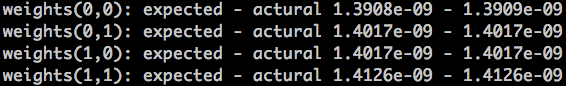
\includegraphics[width=0.8\textwidth]{Lstm11.png}


\section{GRU}\label{Lstm:16}

前面我们讲了一种普通的LSTM,事实上LSTM存在很多\textbf{变体},许多论文中的LSTM都或多或少的不太一样。在众多的LSTM变体中,\textbf{GRU (Gated Recurrent Unit)}也许是最成功的一种。它对LSTM做了很多简化,同时却保持着和LSTM相同的效果。因此,GRU最近变得越来越流行。

GRU对LSTM做了两个大改动:

\begin{enumerate}
	\item
	      将输入门、遗忘门、输出门变为两个门:更新门(Update Gate)\({z}_t\)和重置门(Reset Gate)\({r}_t\)。
	\item
	      将单元状态与输出合并为一个状态:\({h}\)。
\end{enumerate}

GRU的前向计算公式为:
\begin{align*}
	{z}_t         & =\sigma(W_z\cdot[{h}_{t-1},{x}_t])               \\
	{r}_t         & =\sigma(W_r\cdot[{h}_{t-1},{x}_t])               \\
	{\tilde{h}}_t & =\tanh(W\cdot[{r}_t\circ{h}_{t-1},{x}_t])        \\
	{h}           & =(1-{z}_t)\circ{h}_{t-1}+{z}_t\circ{\tilde{h}}_t
\end{align*}


图\ref{fig:Lstm12}是GRU的示意图:

\begin{figure}[!h]
	\centering
	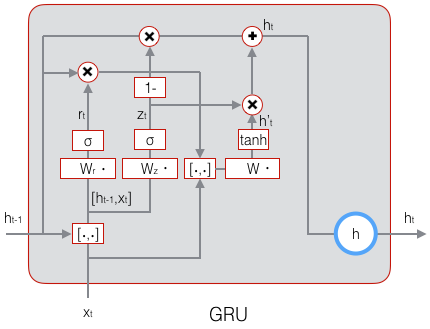
\includegraphics[width=0.6\textwidth]{Lstm12.png}
	\caption{GRU}
	\label{fig:Lstm12}
\end{figure}

GRU的训练算法比LSTM简单一些,留给读者自行推导,本文就不再赘述了。

\section{小结}

至此,LSTM---也许是结构最复杂的一类神经网络---就讲完了,相信拿下前几篇文章的读者们搞定这篇文章也不在话下吧!现在我们已经了解\textbf{循环神经网络}和它最流行的变体---\textbf{LSTM},它们都可以用来处理序列。但是,有时候仅仅拥有处理序列的能力还不够,还需要处理比序列更为复杂的结构(比如树结构),这时候就需要用到另外一类网络:\textbf{递归神经网络(Recursive Neural Network)},巧合的是,它的缩写也是\textbf{RNN}。在下一篇文章中,我们将介绍\textbf{递归神经网络}和它的训练算法。现在,漫长的烧脑暂告一段落,休息一下吧:)






